\documentclass[tikz,border=10pt]{standalone}
\usepackage{mathabx}
\usepackage{stackengine}
\usetikzlibrary{backgrounds}
\usepackage{newunicodechar}
\newunicodechar{♮}{$\natural$}
\newunicodechar{♭}{$\flat$}
\newunicodechar{♯}{$\sharp$}
\newunicodechar{➚}{$\nearrow$}
\newunicodechar{➘}{$\searrow$}
\newunicodechar{ʼ}{'}
\newunicodechar{Ȧ}{\stackon[0.8pt]{A}{.}}
\newunicodechar{Ḃ}{\stackon[0.8pt]{B}{.}}
\newunicodechar{Ċ}{\stackon[0.8pt]{C}{.}}
\newunicodechar{Ḋ}{\stackon[0.8pt]{D}{.}}
\newunicodechar{Ė}{\stackon[0.8pt]{E}{.}}
\newunicodechar{Ḟ}{\stackon[0.8pt]{F}{.}}
\newunicodechar{Ġ}{\stackon[0.8pt]{G}{.}}


\def\centerarc[#1](#2)(#3:#4:#5);%
{
  \draw[#1]([shift=(#3:#5)]#2) arc (#3:#4:#5);
}


\begin{document}
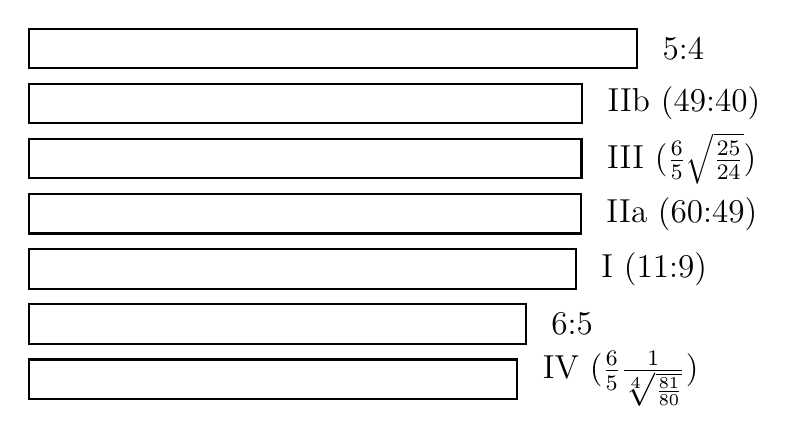
\begin{tikzpicture}

\draw[thick] (0.0, -0.25) -- (6.2051063, -0.25) -- (6.2051063, 0.25) -- (0.0, 0.25) --  cycle;
\node[anchor=west] at (6.4051065, 0.0) { \large IV ($\frac{6}{5}\frac{1}{\sqrt[4]{\frac{81}{80}}}$) };
\draw[thick] (0.0, 0.45000002) -- (6.312631, 0.45000002) -- (6.312631, 0.95) -- (0.0, 0.95) --  cycle;
\node[anchor=west] at (6.5126314, 0.7) { \large 6:5 };
\draw[thick] (0.0, 1.15) -- (6.947943, 1.15) -- (6.947943, 1.65) -- (0.0, 1.65) --  cycle;
\node[anchor=west] at (7.147943, 1.4) { \large I (11:9) };
\draw[thick] (0.0, 1.85) -- (7.0121207, 1.85) -- (7.0121207, 2.3500001) -- (0.0, 2.3500001) --  cycle;
\node[anchor=west] at (7.212121, 2.1000001) { \large IIa (60:49) };
\draw[thick] (0.0, 2.55) -- (7.0193343, 2.55) -- (7.0193343, 3.05) -- (0.0, 3.05) --  cycle;
\node[anchor=west] at (7.2193346, 2.8) { \large III ($\frac{6}{5}\sqrt{\frac{25}{24}}$) };
\draw[thick] (0.0, 3.25) -- (7.026544, 3.25) -- (7.026544, 3.75) -- (0.0, 3.75) --  cycle;
\node[anchor=west] at (7.2265444, 3.5) { \large IIb (49:40) };
\draw[thick] (0.0, 3.95) -- (7.7260346, 3.95) -- (7.7260346, 4.4500003) -- (0.0, 4.4500003) --  cycle;
\node[anchor=west] at (7.9260345, 4.2000003) { \large 5:4 };
\end{tikzpicture}
\end{document}